\documentclass[letterpaper, 10pt]{article}
\usepackage[activate={true,nocompatibility},final,tracking=true,kerning=true,spacing=true,factor=1100,stretch=10,shrink=10]{microtype}
\title{Protocolo de trabajo terminal}
\usepackage[spanish]{babel} %Indica que escribiremos en español
\usepackage[utf8]{inputenc} %Indica qué codificación se está usando ISO-8859-1(latín1)  o utf8  
\usepackage{amsmath} % Comandos extras para matemáticas (cajas para ecuaciones, etc)
\usepackage{amssymb} % Símbolos matemáticos (por lo tanto)
\usepackage{graphicx} % Incluir imágenes en LaTeX
\usepackage{color} % Para colorear texto
\usepackage{subfigure} % subfiguras
\usepackage{float} %Podemos usar el especificador [H] en las figuras para que se
% queden donde queramos
\usepackage{capt-of} % Permite usar etiquetas fuera de elementos flotantes
% (etiquetas de figuras)
\usepackage{sidecap} % Para poner el texto de las imágenes al lado
	\sidecaptionvpos{figure}{c} % Para que el texto se alineé al centro vertical
\usepackage{caption} % Para poder quitar numeración de figuras
\usepackage{commath} % funcionalidades extras para diferenciales, integrales,
% etc (\od, \dif, etc)
\usepackage{cancel} % para cancelar expresiones (\cancelto{0}{x})

\usepackage{blindtext}
\usepackage{multicol} 

\usepackage{anysize} 					% Para personalizar el ancho de  los márgenes
\marginsize{2.54cm}{2.54cm}{2.54cm}{2.54cm} % Izquierda, derecha, arriba, abajo
\usepackage[colorlinks=true,plainpages=true,citecolor=blue,linkcolor=blue]{hyperref}
\usepackage{mathptmx}
\usepackage[T1]{fontenc}\usepackage{pslatex}

% Bibliografía
\usepackage[
sorting=ynt
]{biblatex} %Imports biblatex package
\addbibresource{bibliografia/bibliografia.bib} %Import the bibliography file

% Tamaño de fuente
\newdimen\tamanyo
\newdimen\interlinea
\def\letra#1#2{%
\tamanyo=#1%
\interlinea=1.2\tamanyo%
\fontfamily{ptm}
\fontsize{\the\tamanyo}%
{\the\interlinea}\selectfont#2}

\hypersetup{
	pdftoolbar=true,        % show Acrobat’s toolbar?
	pdfmenubar=true,        % show Acrobat’s menu?
	pdffitwindow=false,     % window fit to page when opened
	pdfstartview={FitH},    % fits the width of the page to the window
	pdftitle={Sistema de predicción enfocado a procesos electorales con base en la socio-física},    % title
	pdfauthor={Josué David Hernandez Ramirez},     % author
	pdfsubject={TTR},   % subject of the document
	pdfcreator={Josué David Hernández Ramírez},   % creator of the document
	pdfproducer={XELATEX}, % producer of the document
	%pdfkeywords={análisis de imagenes} {glucometro} {glucosas} {aplicaciones m\'oviles} 
}


\begin{document}
\begin{center}
    \letra{14pt}{\textbf{Sistema de predicción enfocado a procesos electorales con base en la socio-física}}\\
    \letra{12pt}{\textbf{\textit{Trabajo terminal No. -}}} \\
    \letra{12pt}{\textit{Alumnos: Hernández Ramírez Josué David}} \\
    \letra{12pt}{\textit{Directores: Dr. Ramírez Díaz Mario Humberto}} \\
    \letra{12pt}{\textcolor{black}{\textit{*email: \url{josuehernandezr1605@alumno.ipn.mx}}}}
\end{center}
\newline
\textbf{Resumen -} El presente trabajo terminal propone usar el enfoque socio físico para la predicción de resultados en los procesos electorales, teniendo como guía los trabajos de Galam. Se realizará un sistema computacional que refleje los resultados teóricos propuestos por Galam enfocando los algoritmos socio físicos a este tema. El sistema computacional tiene como objetivo el calcular predicciones de procesos electorales usando formulas matemáticas y autómatas celulares.
\newline
\textbf{Palabras clave -} Física, Matemáticas, Minería de datos, Política, Socio-física, Autómata celular.

\section{Introducción}

La socio-físico es una nueva rama interdisciplinaria de la física que aboga por el uso de los métodos y conceptos de la física de sistemas complejos para el estudio de interacciones colectivas en sociedades y de los fenómenos sociales como propiedades emergentes de un conjunto de individuos. \cite{MarioH.RamirezDiaz2014} 
\newline
\newline
Con los conceptos que existen relacionados a la socio física actualmente que cubren varios temas como: redes sociales, evolución de los lenguajes, dinamismo de la población, crecimiento epidemiológico, terrorismo, elecciones electorales entre otros, se desarrollará un sistema computacional enfocado a resolver el problemas de las elecciones electorales relacionados con el éxito o fracaso de estas. \cite{Galam.1986}

\section{Objetivo}
Desarrollar un sistema de cálculo basado en el enfoque de socio-físico que permita realizar predicciones de resultados en los procesos electorales. 
%, estas predicciones están basadas en datos recolectados con el Programa de Resultados Electorales Preliminares de elecciones anteriores.

\section{Justificación}

La aplicación de la teoría de la socio-física en el ámbito político de México nos ayudaría a tener un panorama mas claro sobre las predicciones electorales con base a los datos recolectados de elecciones anteriores para estimar el grado de aceptación para un partido político determinado.
\newline
\newline
Para los políticos puede proporcionar resultados estimados sobre la confiabilidad y aceptación en un proceso electoral mediante la socio-física y no solamente probabilísticos.

\section{Productos o Resultados esperados}
El producto final será:
\begin{itemize}
    \item Sistema computacional
    \item Manual de usuario
\end{itemize}

\section{Metodología}

Para este trabajo terminal se utilizará la metodología de desarrollo rápido de aplicaciones (DRA), dado que el tiempo de desarrollo es corto, esta metodología permite centrarse en el producto final, hace hincapié en el desarrollo de prioridades y la definición de los plazos de entrega, si estos empiezan a atrasarse permite la reducción de requisitos para el ajuste y de esta manera no aumentar la fecha limite de entrega. Por otro lado la participación de los usuarios es necesaria para el diseño del sistema.\cite{dra}
\begin{figure}[!ht]
    \centering
    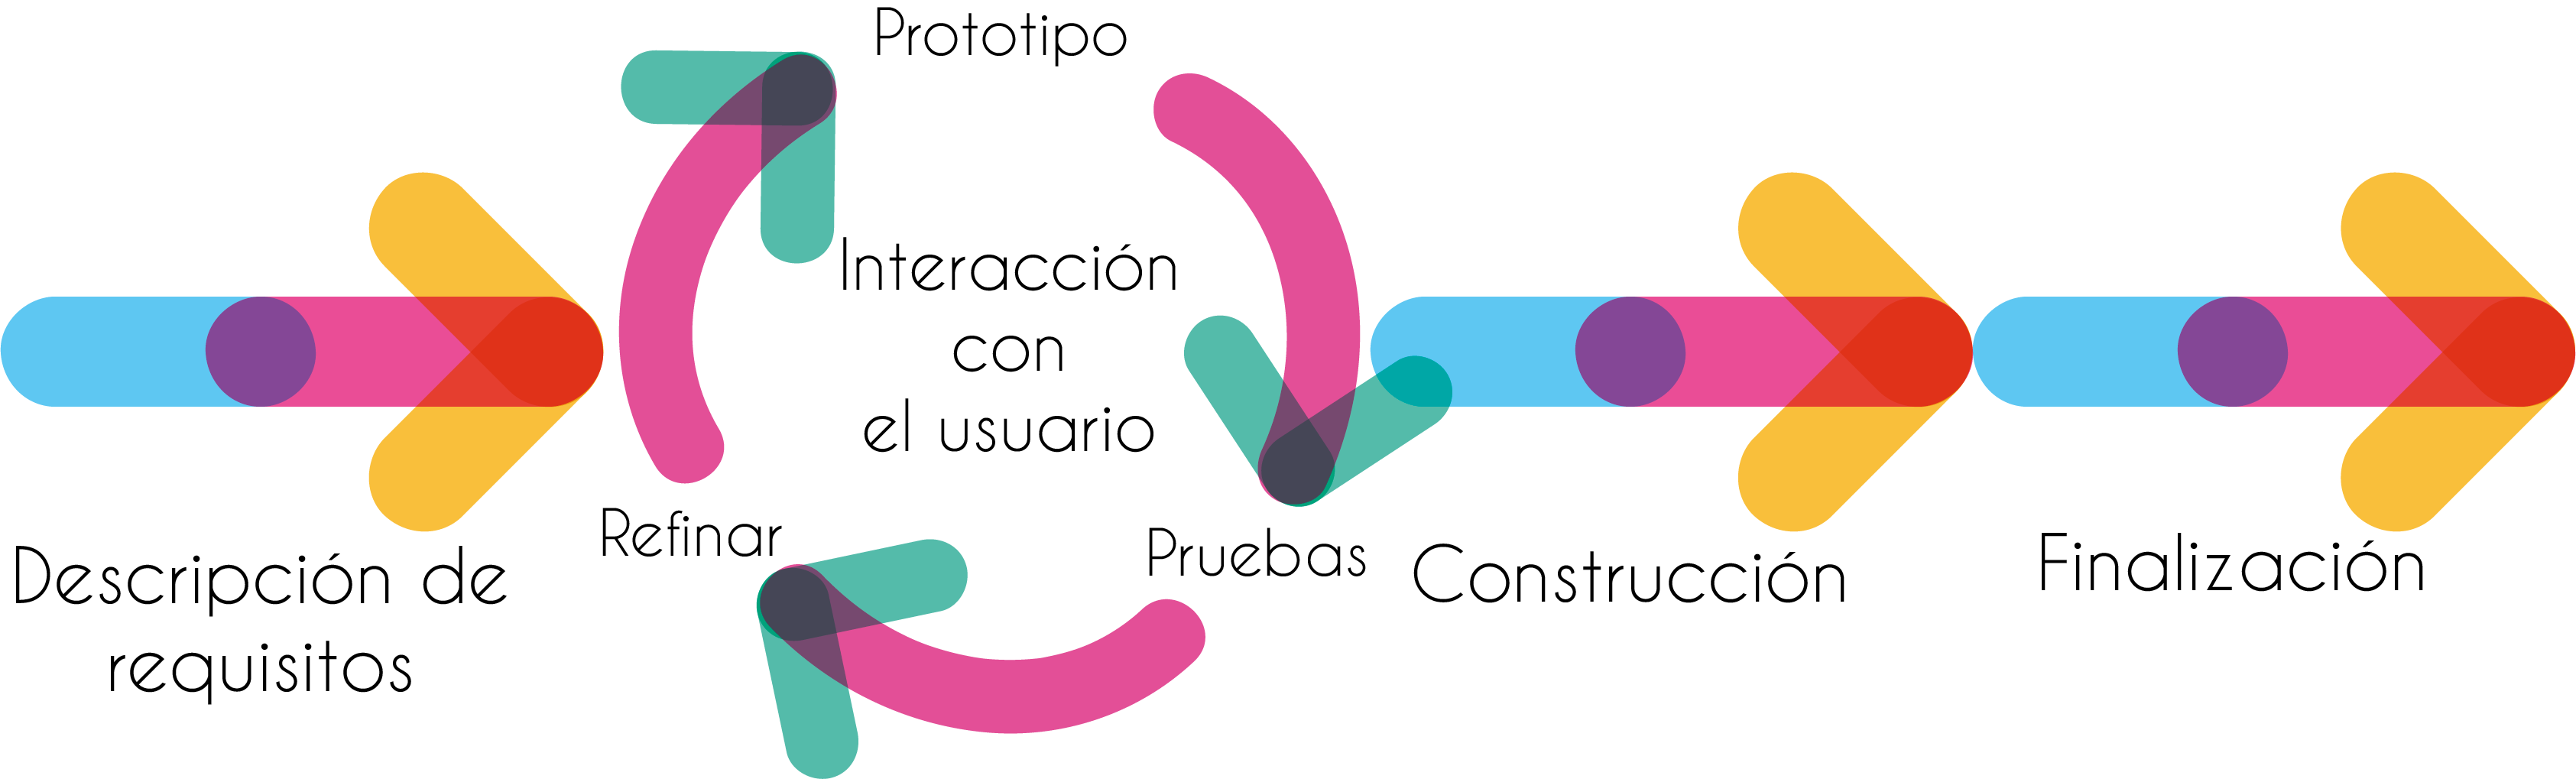
\includegraphics[scale=0.50]{Protocolo/images/4x/RAD@4x.png}
    \caption{Desarrollo rápido de aplicaciones}
    \label{graphic:PRecordatorio}
\end{figure}

\newpage
\section{Cronograma}
\newline
Nombre del alumno: \textit{Hernández Ramírez Josué David}
Título del TT: Sistema de predicción enfocado a procesos electorales con base en la socio-física.
\newpage
\section{Referencias}
\printbibliography[heading=none] %Prints bibliography
\section{Alumnos y directores}

\begin{multicols*}{2}
    \textit{Hernández Ramírez Josué David.- }Alumno de la carrera de Ingeniería en Sistemas Computacionales en la Escuela Superior de Cómputo, Especialidad Sistemas, Boleta: 2017630771, Tel. 7712413847, email \url{jhernandezr1605@alumno.ipn.mx} \\ \\
    
    Firma: \rule{7cm}{1pt}
    \vspace{5mm} %5mm vertical space
    \\
    \textit{Ramírez Díaz Mario Humberto.- }Doctor en Física Educativa, Maestro en Ciencias con Especialidad en Física y actualmente es profesor titular en el Departamento de Posgrado (Maestría en Ciencias en Física Educativa) del Centro de Investigación en Ciencia Aplicada y Tecnología Avanzada de Instituto Politécnico Nacional de México, Áreas de interés incluyen, email \url{mramirezd@ipn.mx} \\ \\
    
    Firma: \rule{7cm}{1pt}
\end{multicols*}

\end{document}